\documentclass[12pt,twoside]{report}
\usepackage{amsmath}
\usepackage{graphicx}
\usepackage{ae}
\usepackage{float}
\usepackage[T1]{fontenc}
\usepackage[utf8]{inputenc}
\usepackage{hyperref}% Links no documento
\usepackage{graphicx}
%\renewcommand{\rmdefault}{phv} % Arial
\usepackage{setspace}
\renewcommand{\baselinestretch}{1.5}
\usepackage{booktabs}
\setlength{\parindent}{1cm}
\usepackage{siunitx}
\usepackage[portuguese]{babel}
\usepackage[euler]{textgreek}
\usepackage{gensymb}
\usepackage{fancyhdr}

\fancypagestyle{plain}{%
	\fancyhf{}
	\fancyhead[R]{\thepage}
	\renewcommand{\headrulewidth}{0pt}
    \onehalfspacing
}
\usepackage{indentfirst}
\usepackage[top = 3cm, bottom = 2cm, left = 3cm, right = 2cm,asymmetric]{geometry}
\AtBeginDocument{\renewcommand{\contentsname}{\centerline{Sumário}}}
\AtBeginDocument{\renewcommand{\bibname}{Referências Bibliográficas}}
\usepackage{titletoc}
\usepackage{titlesec}
\titleformat{\chapter}{\normalfont \titlefont \bfseries}{\thechapter}{1em}{}
\titleformat{\section}{\normalfont \sectionfont \bfseries}{\thesection}{1em}{}
\titleformat{\subsection}{\normalfont \subsectionfont \bfseries}{\thesubsection}{1em}{}
\titleformat{\subsubsection}{\normalfont \subsubsectionfont \bfseries}{\thesubsubsection}{1em}{}
\titlespacing*{\chapter}{0pt}{3.5ex plus 1ex minus .2ex}{2.3ex plus .2ex}
\dottedcontents{chapter}[1.5em]{\bfseries}{1.3em}{.6em}
\dottedcontents{section}[3.0em]{\bfseries}{2em}{.6em}
\dottedcontents{subsection}[4.5em]{\bfseries}{2.7em}{.6em} 
\dottedcontents{subsubsection}[6.0em]{\bfseries}{3.4em}{.6em} 
\newcommand{\titlefont}{\fontsize{14}{20}}
\newcommand{\sectionfont}{\fontsize{12}{20}}
\newcommand{\subsectionfont}{\fontsize{12}{20}}
\newcommand{\subsubsectionfont}{\fontsize{12}{20}}
%%\usepackage[num]{abntex2cite}
%%\citebrackets[]
\renewcommand{\figurename}{Figura}
\renewcommand{\tablename}{Tabela}
\usepackage{chngcntr}
\counterwithout{figure}{chapter}
\counterwithout{table}{chapter}
\usepackage{multirow}
\usepackage{siunitx}
\usepackage{titlesec}
\providecommand{\keywords}[1]{\textbf{{Keywords:}} #1}
\providecommand{\palavraschave}[1]{\textbf{{Palavras-chave:}} #1}
\usepackage[normalem]{ulem}
\useunder{\uline}{\ul}{}
\raggedbottom

\usepackage{gensymb}

\usepackage{xcolor}

\definecolor{COR}{HTML}{FF00FF}

%\newcommand{\x}{$\times$}
%\newcommand{\x}{$\circ$}
\newcommand{\x}{$\bullet$}
%\newcommand{\x}{$\ast$}
%\newcommand{\x}{$\star$}

%\usepackage{lmodern}
\usepackage{slantsc}
\usepackage{footnote}
\usepackage{caption} 


	\definecolor{coda}{rgb}{0,0.3,0.6}
\definecolor{codi}{rgb}{0.6,0.3,0}

\definecolor{0DF}{HTML}{00DDFF}
\definecolor{0FD}{HTML}{00FFDD}
\definecolor{DF0}{HTML}{DDFF00}
\definecolor{FD0}{HTML}{FFDD00}
\definecolor{F0D}{HTML}{FF00DD}
\definecolor{D0F}{HTML}{DD00FF}

\definecolor{0BD}{HTML}{00BBDD}
\definecolor{0DB}{HTML}{00DDBB}
\definecolor{BD0}{HTML}{BBDD00}
\definecolor{DB0}{HTML}{DDBB00}
\definecolor{D0B}{HTML}{DD00BB}
\definecolor{B0D}{HTML}{BB00DD}

\definecolor{09B}{HTML}{0099BB}
\definecolor{0B9}{HTML}{00BB99}
\definecolor{9B0}{HTML}{99BB00}
\definecolor{B90}{HTML}{BB9900}
\definecolor{B09}{HTML}{BB0099}
\definecolor{90B}{HTML}{9900BB}

\definecolor{079}{HTML}{007799}
\definecolor{097}{HTML}{009977}
\definecolor{790}{HTML}{779900}
\definecolor{970}{HTML}{997700}
\definecolor{907}{HTML}{990077}
\definecolor{709}{HTML}{770099}

\definecolor{057}{HTML}{005577}
\definecolor{075}{HTML}{007755}
\definecolor{570}{HTML}{557700}
\definecolor{750}{HTML}{775500}
\definecolor{705}{HTML}{770055}
\definecolor{507}{HTML}{550077}

\definecolor{035}{HTML}{003355}
\definecolor{053}{HTML}{005533}
\definecolor{350}{HTML}{335500}
\definecolor{530}{HTML}{553300}
\definecolor{503}{HTML}{550033}
\definecolor{305}{HTML}{330055}

\definecolor{013}{HTML}{001133}
\definecolor{031}{HTML}{003311}
\definecolor{130}{HTML}{113300}
\definecolor{310}{HTML}{331100}
\definecolor{301}{HTML}{330011}
\definecolor{103}{HTML}{110033}

\definecolor{strs}			{rgb}	{0.9,	0.2,	0	}
\definecolor{coments}		{rgb}	{0,		0.5,	0	} 
\definecolor{backcode}		{rgb}	{0.3,	0,		0.2	}
\usepackage{listings}%Configura layout para mostrar codigos a partir de arquivo
\lstset{% Configurando layout para mostrar codigos C++
	language=C++,
	basicstyle=\ttfamily\small\setstretch{1}, 
	keywordstyle=[1]\color{079}, 
	keywordstyle=[2]\color{907},
	keywordstyle=[3]\color{097},
	keywordstyle=[4]\color{790},
	stringstyle=\color{strs}, 
	commentstyle=\color{coments},
	morekeywords=[1]{byte, once, sizeofV},
	morekeywords=[2]{HeapSort, QuickSort, MergeSort, Sort, qSort, InsertSort, QuickSortCentral, QuickSortRandom, SelectSort, RadixSort, BubbleSort, BeadSort},
	morekeywords=[3]{cout, fout, endl},
	morekeywords=[4]{Tipo, Size},
	tabsize=2,
	extendedchars=true, 
	showspaces=false, 
	showstringspaces=false, 
	frame=L,
	numbers=left,
	numberstyle=\tiny,
%	firstnumber=last,
	breaklines=true, 
	backgroundcolor=\color{backcode!5},
	breakautoindent=true, 
	captionpos=b,
	xleftmargin=0pt,
}

\setcounter{tocdepth}{4} % Níveis exibidos no sumário
\setcounter{secnumdepth}{4} % Nível de números exibidos

\usepackage{lipsum}
\usepackage{makecell}

\newcommand{\autor}{Heitor Rodrigues Savegnago\\Allan de Moraes Navarro}
\newcommand{\titulo}{Comparação entre algoritmos de ordenação}
\newcommand{\local}{Santo André - SP}
\newcommand{\data}{2017}
\newcommand{\notaDeRosto}
{
	\hspace{.45\textwidth} % posicionando a minipage
    \begin{minipage}{.5\textwidth}
      \singlespace
      Palavras
    \end{minipage}
}



\begin{document}
	\begin{titlepage}
      \center
      {\large UNIVERSIDADE FEDERAL DO ABC}\\[4cm]
      {\large \autor}\\[4cm]
      {\Large \bf \titulo }\\\vfill
      {\local\\\data}
	\end{titlepage}
%    \begin{titlepage}
%      \center
%      {\large \autor}\\[7cm]
%      {\Large \bf \titulo}\\[2cm]
%      {\notaDeRosto}\\\vfill
%      {\local\\\data}
%	\end{titlepage}
       
	\pagenumbering{arabic}
    \pagestyle{empty}
	    
	\chapter{Resultados}
	
	Os resultados dos processamentos de cada algoritmo de ordenação é apresentado na figura \ref{Graph}. Além dos métodos indicados na proposta de projeto, também foram analisadas situações onde o \lstinline|QuickSort| tem pivô central e pivô aleatório.
	
	\begin{figure}[!h]
		\begin{center}
			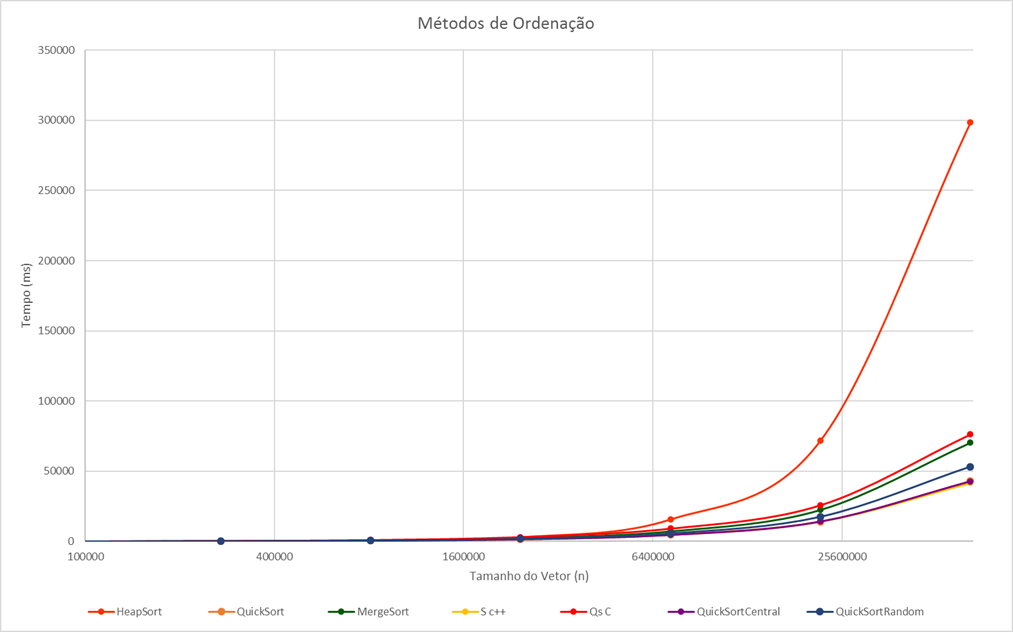
\includegraphics[width=\textwidth]{../Grafico.png}
			\caption{Gráfico comparativo para os algoritmos.}
			\label {Graph}
		\end{center}
	\end{figure}
	
	\chapter{O Código}
	
	Os métodos selecionados foram:
	
	\begin{itemize}
		\item \lstinline|HeapSort|;
		\item \lstinline|QuickSort|, com pivô no primeiro item;
		\item \lstinline|MergeSort|;
		\item \lstinline|Sort|, função da biblioteca \lstinline|algorithm|;
		\item \lstinline|qSort|, função da biblioteca \lstinline|cstdio|;
		\item \lstinline|InsertSort|
		\item \lstinline|QuickSort|, com pivô no item centra;
		\item \lstinline|QuickSort|, com pivô em item aleatório;
		\item \lstinline|SelectSort|;
		\item \lstinline|RadixSort|;
		\item \lstinline|BubbleSort|;
		\item \lstinline|BeadSort|.
	\end{itemize}

	Infelizmente nem todos os métodos puderam ser analisados devido ao tempo de processamento.
	
	O código fonte do programa utilizado para a verificação dos métodos é apresentado aqui, mas também está disponível em um diretório do \lstinline|GitHub|, acessível pelo endereço apresentado na figura \ref{QR}

	\begin{figure}[!h]
		\begin{center}
			
\includegraphics[width=.5\textwidth]{../QR.png}
			\caption{Código QR para acesso do link \href{	https://github.com/HeckRodSav/ProjAED}{\lstinline|github.com/HeckRodSav/ProjAED|}.}
			\label {QR}
		\end{center}
	\end{figure}
	
	
	\section{Estrutura principal}
	
	\lstinputlisting{../ProjAED/ProjAED.cpp}
	
	\section{Classe com ordenadores}

	\lstinputlisting{../ProjAED/Ordem.cpp}
	
	
\end{document}